\chapter{Conexión por caminos}%
\label{cha:conexion_por_caminos}
La conexión por caminos va a ser un elemento central sobre todo en la parte de topología algebraica posterior. Es similar al concepto de conexión que hemos visto, pero la diferencia es que introducimos un elemento ``conector'': los caminos.

\begin{defi}[Camino]
Sea $X$ un espacio topológico, definimos un \textbf{camino en $X$} como una aplicación continua $\alpha: \left[ a, b \right] \subset \mathbb{R}_u \rightarrow X$ y decimos que:
\begin{itemize}
    \item Los puntos $\alpha\left( a \right)$ y $\alpha\left( b \right)$ son los extremos inicial y final del camino.
    \item La imagen $\alpha\left[ a, b \right] \subset X$ es\footnote{Nótese que la traza es un conexo, pues es imagen continua del conexo $[a,b]$.} la \textbf{traza}.
\end{itemize}
\end{defi}

\begin{prop}[Cambios de parámetros]
Sea $X$ un espacio topológico, $\alpha :[a,b] \rightarrow X$ un camino en él y $\varphi
 : [c,d]\rightarrow [a,b]$ una aplicación, entonces:
\begin{itemize}
\item Si $\varphi$ es continua, la aplicación $\alpha \circ \varphi :[c,d]\rightarrow X$ es otro camino sobre $X$ con la misma traza que $\alpha$.
\item Si $\varphi$ es un homeomorfismo\footnote{En funciones de un variable, la equivalencia a ser homeomorfismo (biyectiva, continua y continua la inversa) es ser una función continua y monótona.}, la aplicación $\alpha \circ \varphi:[c,d]\rightarrow X$ es exactamente el mismo camino que $\alpha$, pero con parametrización distinta.
\end{itemize}
al último resultado se le conoce como \textbf{cambio de parámetro}.
\begin{figure}[H]
    \centering
    \incfig[0.8]{cambio-de-caminos}
    \caption{\textit{Ejemplo de un cambio de parámetros para un camino.}}
    \label{fig:cambio-de-caminos}
\end{figure} 
\end{prop}

\begin{obs}
Es importante tener en cuenta que sólo se trata del mismo camino cuando $\varphi$ es homeomorfismo. La principal diferencia está en que cuando $\varphi$ es sólo continua, se conserva la traza, pero no la velocidad a la que se recorre.
\end{obs}

\begin{ej}
Un cambio de parámetro muy útil en lo que queda de documento va a ser la interpolación lineal, que consiste en la parametrización de cualquier segmento en términos del segmento $[0,1]$. El cambio, considerando $p, q\in \mathbb{R}^n$, viene dado por la siguiente aplicación:
\begin{align*}
\varphi : [0, 1] &\longrightarrow [p, q] \\
			t & \longmapsto (1-t)p + tq
\end{align*}
Este resultado es muy potente porque permite reducir cualquier camino a uno parametrizado en $[0,1]$, lo que será de gran utilidad en los capítulos posteriores.
\end{ej}

\begin{defi}[Producto de caminos]
Sea $X$ un espacio topológico y $\alpha : [a,b]\rightarrow X$ y $\beta:[c,d]\rightarrow X$ dos caminos tales que $\alpha(b) = \beta(c)$, entonces la aplicación:
\begin{align*}
\alpha \ast \beta : [a,b] \cup [c,d] &\longrightarrow X \\
						t &\longmapsto \begin{cases}
										\alpha(t) & t \in [a,b] \\
										\beta(t) & t\in [c,d]
										\end{cases}	
\end{align*}
es el camino que resulta de unir los caminos $\alpha$ y $\beta$.
\begin{figure}[H]
    \centering
    \incfig[0.8]{producto-de-caminos}
    \caption{\textit{Ejemplo de un producto de caminos}}
    \label{fig:producto-de-caminos}
\end{figure}
\end{defi}

\begin{obs}
Una alternativa para ver mejor que se trata de un camino es reparametrizar el camino $\beta$ al intervalo $[b,b+(d-c)]$. Como $\beta(b) = \alpha(b)$, el camino $\alpha \ast b$ definido en $[a,b+(d-c)]$ ahora ya tiene un aspecto más uniforme que el de la definición.
\end{obs}

\begin{ej}
Si hacemos el producto de segmentos consecutivos obtenemos \textbf{caminos poligonales}. 
\end{ej}

\section{Mantras y propiedades}%
\label{sec:conexion_por_caminos}
Una vez definidos los conectores fundamentales que serán los caminos, ahora sí podemos estudiar qué significa estár conectado por caminos y qué consecuencias tiene con respecto a la conexión y las propiedades del espacio.

\begin{defi}[Conexión por caminos]
Sea $X$ un espacio topológico, decimos que es \textbf{conexo por caminos} si y sólo si 
\[
\forall x, y \in X,\ \exists \sigma: \left[ a, b \right] \rightarrow X,\ \sigma\left( a \right) = x\; \land \;\sigma\left( b \right) = y
\]
cualesquiera dos de sus puntos se pueden conectar con un camino.
\end{defi}

\begin{obs}
Fijemos un $x_0\in X$ y consideremos $\sigma_x : [a,b]\rightarrow X$ tal que $\sigma_x(a) = x_0$ y $\sigma_x(b) = x$. Como la traza de $\sigma_x$ hemos comentado que es conexa y podemos escribir\footnote{En este caso, $\sigma_x$ es un abuso de notación para escribir que es la traza de $\sigma_x$.} $X = \bigcup_{x\in X} \sigma_x$, el conjunto $X$ es conexo por el teorema del pivote (pues todos los $\sigma_x$ intersecan en $x_0$).
\end{obs}

\begin{ej}
\begin{enumerate}
    \item La mayor parte de los conexos conocidos son conexos por caminos:
    \begin{itemize}
        \item Los abiertos conexos de la topología usual son conexos por poligonales, que son caminos.
        \item Los conjuntos convexos y los estrellados también son conexos (casi por definición se prueba).
    \end{itemize}
    \item El seno del topólogo $\Gamma$ es la traza de $\alpha\left( t \right) = \left( t, \sin\frac{1}{t} \right) : t > 0$ y es conexo tanto él como su adherencia $\overline{\Gamma} = J \cup \Gamma$ donde $J = \{0\} \times \left[ 0, 1 \right]$. Sin embargo, la adherencia $\overline{\Gamma}$ sirve como contraejemplo para ver un conjunto conexo que no es conexo por caminos.
    \begin{demo}
    Fundamentalmente hay que demostrar que no todos los puntos están conectados por caminos. En particular, vamos a demostrar que no existen caminos que $\sigma: \left[ a, b \right] \rightarrow \overline{\Gamma}$ donde $\sigma\left( a \right) = p \in J$ y $\sigma\left( b \right) = q \in \Gamma$, es decir, al intentar buscar un camino de $J$ a $\Gamma$ la cosa se estropea.
    \begin{figure}[H]
        \centering
        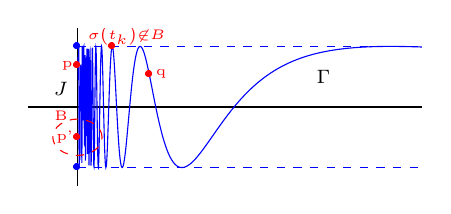
\begin{tikzpicture}
        \begin{axis}[
            axis lines* = middle,
            height=2cm,
            width=5cm,
            scale only axis=true,
            ytick=\empty,
            xtick=\empty,
            xmin=-0.1,
            xmax=0.7,
            ymin=-1.3,
            ymax=1.3,
        ]
        \addplot[
            domain=0.001:0.8,
            samples=1000,
            color=blue,
            smooth,
        ]
        {sin(deg(1/x))};
        \draw[blue, dashed] (0,1) -- (1,1);
        \draw[blue, dashed] (0,-1) -- (1,-1);
        \node at (0,0.3) [left] {\scriptsize $J$};
        \node[blue] at (0,1) {\tiny \textbullet};
        \node[blue] at (0,-1) {\tiny \textbullet};

        \node[red] at (0.01,0.68) [left] {\tiny p};
        \node[red] at (0,0.7) {\tiny \textbullet};

        \node[red] at (0.01,-0.5) [left] {\tiny p'};
        \node[red] at (0,-0.5) {\tiny \textbullet};

        \draw[red, dashed] (0,-0.5) ellipse (0.05 and 0.3);
        \node[red] at (0, -0.15) [left] {\tiny B};

        \node[red] at (0.071,1) {\tiny \textbullet};
        \node[red] at (0.1,0.85) [above] {$\scriptscriptstyle \sigma\left( t_k \right) \not\in B$};

        \node[red] at (0.146,0.55) {\tiny \textbullet};
        \node[red] at (0.14,0.55) [right] {\tiny q};

        \node at (0.5, 0.5) {\scriptsize $\Gamma$};
        \end{axis}
        \end{tikzpicture}
        \caption{\textit{La bola representada es de radio pequeño.}}
        \label{fig:seno_topologo_caminos}
    \end{figure}
    
	Supongamos que sí, que existe un camino con $\sigma(0) = p \in J$ y $\sigma(1) = q \in \Gamma$ definido como:
	\begin{align*}
		\sigma : [0, 1] &\longrightarrow \overline{J} \\
					t &\longmapsto (\alpha(t), \beta(t))
	\end{align*}
	entonces el valor $t_0 = \max \{t \in \left[ a, b \right] : \alpha\left( t \right) = 0\}$ existe porque (falta explicación) y es menor estricto que $1$, pues $\sigma(1) = (\alpha(1), \beta(1)) = q \in J \Rightarrow \alpha(1) \neq 0$. Al valor $\sigma(t_0) = (0, \beta(t_0))$ lo denotaremos por $p'$ en lo sucesivo.
	
	   $\Rightarrow \begin{cases}
                \alpha\left( a' \right) = 0,\ \sigma\left( a' \right) = p' \in J\\
                t > a': \alpha\left( t \right) > 0 \Rightarrow \sigma\left( t \right) \in \Gamma \Rightarrow \beta\left( t \right) = \sin \frac{1}{\alpha\left( t \right)} 
            \end{cases} $

            Supongamos $p' = \sigma\left( a' \right) \neq \left( 0, 1 \right)$ (punto) y $\exists \delta: B\left( p', \delta \right) \cap \{y = 1\} = \emptyset$. $\sigma$ continua $\Rightarrow \exists \sigma\left[ a', \varepsilon \right] \subset B\left( p', \delta \right) \Rightarrow \sigma\left[ a', \varepsilon \right] \cap \{y = 1\} = \emptyset$. (si $p' = \left( 0, 1 \right)$ evitaríamos $\{y = -1\}$)

            $\alpha$ continua $\Rightarrow \alpha\left[ a', \varepsilon \right] \subset \mathbb{R}$ conexo compacto $=$ intervalo: $\alpha\left[ a', \varepsilon \right] = \left[ 0, c \right]$.

            La oscilación de $\sin \frac{1}{x}$ lleva $\sigma$ a $\{y = 1\}$, fuera de la bola elegida:
            \begin{align*}
            k \gg 0 &\Rightarrow \frac{2}{\left( 1 + 4k \right) \pi} \in \left[ 0, c \right] = \alpha\left[ a', \varepsilon \right] \Rightarrow \exists a' < t_k < \varepsilon: \alpha\left( t_k \right) = \frac{2}{\left( 1 + 4k \right) \pi}\\ 
                &\Rightarrow \sigma\left( t_k \right) = \left( \alpha\left( t_k \right), \sin\left( \frac{1}{\alpha\left( t_k \right)} \right) \right) = \left( x_k, 1 \right) 
            \bot \end{align*}
    \end{demo}
\end{enumerate}
\end{ej}

Como el concepto también tiene que ver con la conexión de un conjunto y parece muy similar al que hemos comentado, parece razonable que casi todo lo que dijimos acerca de conexión sea válido en este caso.

\begin{theo}[del pivote]
Sea $X$ un espacio topológico, $A$ un subespacio definido como $A = \bigcup_{i} A_i$ donde los $A_i$ son una familia de conexos por caminos de $X$, si $\bigcap_{i} A_i \neq \emptyset$, entonces $A$ es conexo por caminos. 
\end{theo}
\begin{demo}
Demostración por dibujo:
\begin{figure}[H]
    \centering
    \incfig[0.5]{teorema-del-pivote-caminos}
    \caption{\textit{Teorema del pivote con caminos}}
    \label{fig:teorema-del-pivote-caminos}
\end{figure}
\end{demo}

\begin{theo}[Conservación por continuidad]
Sean $X$ e $Y$ espacios topológicos, $f: X \rightarrow Y$ una función continua y $A \subset X$ un conjunto conexo por caminos, entonces $f\left( A \right)$ es conexo por caminos.
\end{theo}
\begin{demo}
De nuevo, ilustramos la demostración con un dibujo:
\begin{figure}[H]
    \centering
    \incfig[0.4]{imagen-conexa-por-caminos}
    \caption{\textit{Imagen continua conexa por caminos}}
    \label{fig:imagen-conexa-por-caminos}
\end{figure}
\end{demo}

\begin{obs}
Uno podría pensar, por la similitud que estamos viendo con la conexión del capítulo anterior, que el teorema sobre la conexión de la adherencia es extensible a la conexión por caminos. Sin embargo ¡Esto no es cierto!

El seno del topólogo $\Gamma$ es conexo por caminos: $\left( a, \sin\frac{1}{a} \right)$ y $\left( b, \sin\frac{1}{b} \right)$ se conectan por el camino evidente, $\alpha\left( t \right) = \left( t, \sin\frac{1}{t} \right),\ a \le t \le b$. Pero, como hemos visto, la adherencia $\overline{\Gamma}$ no es conexa por caminos. 
\end{obs}

\section{Tabla de comportamiento}%
\label{sec:tabla_de_comportamiento_conx_caminos}
En este apartado estudiamos como se comportan la conexión por caminos con respecto a las construcciones del tema \nameref{cha:construcciones} para ver cuándo se conservan, cuándo se pierden y qué podemos añadir para no perderlas.

%TODO: Fix tabla
\begin{table}[H]
\centering
\begin{tabular}{| c | c | c | c | c |}
\hline
& Subespacios & Cocientes & Productos & Sumas\\
\hline
Conexión por caminos & \ding{55} & \checkmark & \begin{tabular}{cc} \checkmark & \checkmark \end{tabular} & \ding{55} \\
\hline
Demostración: Conexo & Continuidad & Prop & ??? \\
\hline
\end{tabular}
\caption{\textit{La tabla nos indica como se conserva la conexión por caminos en las construcciones que hemos visto. Las sumas y los productos son finitos.}}
\end{table}

\begin{prop}[Conservación por producto]
Sean $X$ e $Y$ dos espacios topológicos, el producto $X\times Y$ es conexo por caminos si y sólo si $X$ e $Y$ son conexos por caminos.
\end{prop}
\begin{demo}
\begin{itemize}
\item $\Leftarrow$

Escojamos dos puntos cuales quiera $\left( x_1, y_1 \right),\ \left( x_2, y_2 \right) \in X \times Y$ y veamos que existe un camino que los une. Por la conexión por caminos de cada componente del producto, sabemos que ocurre lo siguiente: 
\[
\begin{cases}
    \sigma: \left[ a, b \right] \rightarrow X: \begin{cases}
        \sigma\left( a \right) = x_1 \\
        \sigma\left( b \right) = x_2
    \end{cases} \\
    \tau: \left[ a, b \right] \rightarrow Y: \begin{cases}
        \tau\left( a \right) = y_1 \\
        \tau\left( b \right) = y_2
    \end{cases}
\end{cases} 
\]
Luego la composición de ambos caminos sobre cada componente como componentes de un camino en el producto necesariamente será un camino que unirá los puntos del inicio.
\[
\gamma = \left( \sigma, \tau \right) : \left[ a, b \right] \rightarrow X \times Y: \begin{cases}
        \gamma\left( a \right) = \left( x_1, y_1 \right)\\
        \gamma\left( b \right) = \left( x_2, y_2 \right)
    \end{cases}  
\]

\item $\Rightarrow$

Como para que una función con varias componentes sea continua cada componente debe ser continua, el proceso de la implicación anterior es completamente reversible porque la existencia de un camino en el producto implica la existencia de un camino en cada componente considerando dicha componente como camino en el factor.
\end{itemize}
\end{demo}


\chapter{Componentes conexas\texorpdfstring{\\}{} por caminos y conexión\texorpdfstring{\\}{} local por caminos}%
\label{cha:componentes_conexas_por_caminos_y_conexion_local_por_caminos}
Del mismo modo que estudiamos en el capítulo de conexión las ``piezas conexas'' en las que se podían dividir los conjuntos que no eran conexos y localizamos la noción de conexión, tiene sentido definir los mismos conceptos para conexión local.

\section{Componentes conexas por caminos}%
\label{sec:componentes_conexas_por_caminos}
La definición y las propiedades de las componentes conexas por caminos serán prácticamente iguales a las de conexión salvo por algún detalle menor. El fundamento de la idea, que es la de subconjunto conexo maximal, sigue siendo el componente básico de la teoría.

\begin{defi}[Componente conexa por caminos]
Sea $X$ un espacio topológico, definimos una \textbf{componente conexa por caminos} como un subconjunto conexo por caminos maximal.
\end{defi}

\begin{prop}[Caracterización de componentes conexas por caminos]
Sea $X$ un espacio topológico y $a\in X$ un punto del mismo, el conjunto:
\[
C_c(a) := \bigcup_{A \ni a} A \mbox{ donde }A \mbox{ es conexo por caminos}
\]
verifica las siguientes propiedades:
\begin{itemize}
\item Es conexo por caminos
\item Para cualquier $E\subset X$ conexo por caminos tal que $E\cap C_c(a) \neq \emptyset$, se cumple que $E\subset C_c(a)$.
\end{itemize}
\end{prop}
\begin{demo}
Si uno se fija en la demostración de la misma proposición para componentes conexas, se dará cuenta que principalmente la herramienta que utiliza es el teorema del pivote y, como hemos demostrado dicho teorema para la conexión por caminos, la demostración es completamente análoga.
\end{demo}

\begin{obs}
De la misma forma que las componentes conexas formaban una partición de $X$, las componentes conexas por caminos formarán una partición de $X$ ¡pero más fina y no necesariamente de cerrados! De nuevo, el seno del topólogo es un buen contraejemplo: si consideramos el espacio $X = \overline{\Gamma}$, los conjuntos $J$ y $\Gamma$ son dos componentes conexas por caminos donde la primera es cerrada y la otra no. Además, $\overline{\Gamma}$ sólo tiene una componente conexa (ella misma), pero acabamos de ver que tiene dos componentes conexas por caminos, luego la partición es más fina.
\end{obs}

\section{Conexión local por caminos}%
\label{sec:conexion_local_por_caminos}
En este caso, también es útil conocer cuándo podemos trabajar de forma local a un punto asumiendo que dicha localización es conexa por caminos y a esto es lo que llamamos conexión local por caminos.

\begin{defi}[Conexión local por caminos]
Sea $X$ un espacio topológico, decimos que es \textbf{localmente conexo por caminos} si y sólo si para todo punto $x\in X$ existe una base de entornos $\mathcal{B}^x$ formada por abiertos conexos por caminos.
\end{defi}

\begin{prop}[Caracterización de la conexión local]
Sea $X$ un espacio topológico, $X$ es localmente conexo por caminos si y sólo si las componentes conexas por caminos de un abierto son abiertas.
\end{prop}
\begin{demo}
De nuevo, las demostraciones son completamente análogas a sus homólogas del capítulo de conexión.
\end{demo}

\begin{obs}
Sin excesiva dificultad, es sencillo demostrar que la definición de conexión local puede prescindir de la apertura de los conexos que forman la base de entornos, esto es, que la definición dada es equivalente a ``$X$ es localmente conexo por caminos si y sólo si $\forall x \in X, \ \exists \mathcal{V}^x$ base de entornos formada por conexos por caminos''
\end{obs}

\section{Tabla de comportamiento}%
\label{sec:tabla_de_comportamiento_conx_local_caminos}
%TODO: Fix tabla
\begin{table}[H]
\centering
\begin{tabular}{| c | c | c | c | c |}
\hline
& Subespacios & Cocientes & Productos & Sumas\\
\hline
Conexión local por caminos & \ding{55} & \checkmark & \checkmark & \checkmark\\
\hline
\end{tabular}
\caption{\textit{También vale que las c.c.c del producto son los productos de las c.c.c de los factores.}}
\end{table}

\section{Relaciones entre las propiedades de conexión}%
\label{sec:relaciones_entre_las_propiedades_de_conexion}
Por las similitudes entre ambos tipos de conexión definidos, no está demás estudiar qué condiciones han de darse para obtener unas a partir de otras y viceversa.

\begin{prop}
Conexo y localmente conexo por caminos $\Rightarrow$ Conexo por caminos.
\end{prop}
\begin{demo}
\begin{itemize}
    \item Conexo $\Rightarrow \forall x, y,\ \exists \text{ cadenas de } x \text{ a } y$.
    \item Localmente conexo por caminos $\Rightarrow$ cadenas de abiertos conexos por caminos $\xRightarrow{\text{Variante del pivote}}$ Estas cadenas son conexas por caminos.
\end{itemize}
Por tanto, $\exists$ camino de $x$ a $y$.
\end{demo}

\begin{obs}[Resumen]
Por especificar todas las posibilidades:
%TODO: Imagen
\begin{center}
    \includegraphics[scale=0.3]{images/resumen_conx} 
\end{center}
\end{obs}

\begin{enun}
Contraejemplos. Los menos fáciles son $*$ y $**$ 
\end{enun}

\begin{ej}
\begin{itemize}
    \item Sea $\left( \mathbb{R}^2, \mathcal{T}_{\text{rad}} \right)$. Veamos si es conexo por caminos porque entonces será conexo.

    %TODO: Dibujo
    Primero intentamos parametrizar por interpolación: $\left( 1 - t \right)a + tb$. Como $\mathcal{T}_{\text{rad}}|_r = \mathcal{T}_{u}|_r$ es correcto el camino ($r$ es una recta).
    En cambio si el camino es una curva cualquiera, la topología relativa es la discreta, es decir, la preimagen de un punto es todo $\left[ 0, 1 \right]$ al ser 
    un abierto y cerrado en un conexo. Por tanto, $f$ será constante (contradicción).

    En definitiva, tomamos como caminos entre dos puntos, la recta que los une. Con esto, el espacio es conexo por caminos $\Rightarrow$ conexo.

    La usual es localmente conexa por caminos. Si en la radial es localmente conexa por caminos tenemos que si $x_0 \in U$ entonces $\exists U \supset V_{\text{ab}} = C_{\text{cam.}} \left( x_0 \right)$es el candidato a entorno abierto conexo por caminos de la base buscada. 

    Usaremos $V = \left\{ x \in U : \exists P \supset U: x_0 \rightarrow x\right\}$ con $P$ poligonal %TODO: Dibujo
    que será conexo por caminos radiales. Veamos que es abierto (radial).

    Esto quiere decir que $\forall x \in V$ se cumple ``la condición radial''.
    %TODO: Dibujo
    $\exists \underbrace{\left( x - \varepsilon, x + \varepsilon \right)}_{\ni y} \subset U \cap L$. Formamos $P_y = P_x \cup \left[ x, y \right] \subset U \Rightarrow \left( x - \varepsilon, x + \varepsilon \right) \subset V \cap L$.

    %TODO: Cambiar de lugar
    \item Veamos ahora la compacidad tenemos que $\mathcal{T}_u \subset \mathcal{T}_r \Rightarrow$ si $K$ compacto en la radial $\Rightarrow$ también lo será en la usual. Por tanto, al no ser $\mathbb{R}^2$ con la usual compacto, tampoco lo será con la radial.

    En cambio como con la usual, $\mathbb{R}^2$ sí es Lindelöf no podemos decidir directamente si con la radial lo es o no. Pero no es así porque las curvas son cerradas pero su topología relativa es la 
    discreta y, por tanto, no son Lindelöf. Como se hereda, la radial no puede ser Lindelöf.

    \item Veamos la compacidad local. No lo es. %TODO: Imagen.
\end{itemize}
\end{ej}
